\subsection{EDA}

EDA provides an overview of what could be done to the data to improve the models' performance. 

\subsubsection{Data Profiling and Malformed Entries}

All of the columns and their data types can be seen at table \ref{tab:columns}. When checking for null values, all other columns are free from it other than \texttt{Income}. Upon inspection, there seems to be no connection with all the other attributes of the entries with null valued `Income`. As far as inspection and analysis goes, they seem to just be malformed entries. 

\texttt{Marital\_Status} also has multiple entries that could be thought of as different, similar, or sometimes even a malformed entry. In the list of unique values for the column, the values are \texttt{Divorced, Single, Married, Together, Widow, YOLO, Alone, Absurd}. Upon listing the value counts, \texttt{Alone, YOLO, Absurd} have very few entries which could be considered as outliers. There are been thoughts of merging some of these entries to the other entries with bigger value counts; e.g. \texttt{Single} would adopt the records with \texttt{Alone}, etc. However the problem lies wherein there is no way to deduce their backgrounds and whether or not the adopting categories should take in the outliers. To further explain, there is no way to tell if a record that is \texttt{Alone} might have came from a divorced background or if they simply are single. However further explanation of the choice between data integrity and model performance would come in later in experimentations

\subsubsection{Univariate Analysis}

The skew and imbalance of data attributes can be seen upon further isolated inspection. Firstly, \texttt{Income}'s central tendencies at table \ref{tab:income desc}

To put into perspective figure \ref{fig:income hist} shows the distance of the max value from the mean of the distribution with a skewness of 6.763487372811116

Depending if the models are robust to outliers, they will be removed, experimentations will further explain these phenomena

\begin{table}[H]
    \caption{Income column's descriptive statistics}
    \label{tab:income desc}
    \centering
    \begin{tabularx}{\linewidth}{l>{\raggedleft\arraybackslash}X}
        \toprule
        Statistic & Value\\
        \midrule
        count & 2216 \\
        mean & 52247.251354\\
        std & 25173.076661\\
        min & 1730\\
        25\% & 35303\\
        50\% & 51381.5\\
        75\% & 68522\\
        max & 666666\\
        \bottomrule
    \end{tabularx}
\end{table}

\begin{figure}[H]
    \centering
    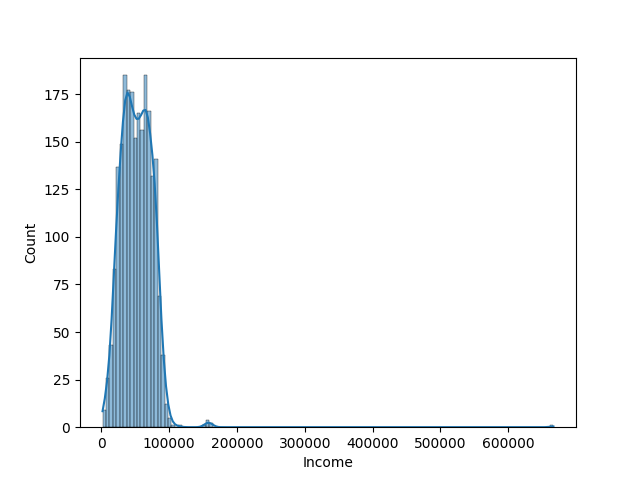
\includegraphics[width=\linewidth]{figures/income_histplot.png}
    \caption{histogram of Income values}
    \label{fig:income hist}
\end{figure}

On the other hand for \texttt{Education} While it could be considered that the \texttt{Basic} records are outliers, removing them may misrepresent the dataset.

% \begin{figure}[H]
%     \centering
%     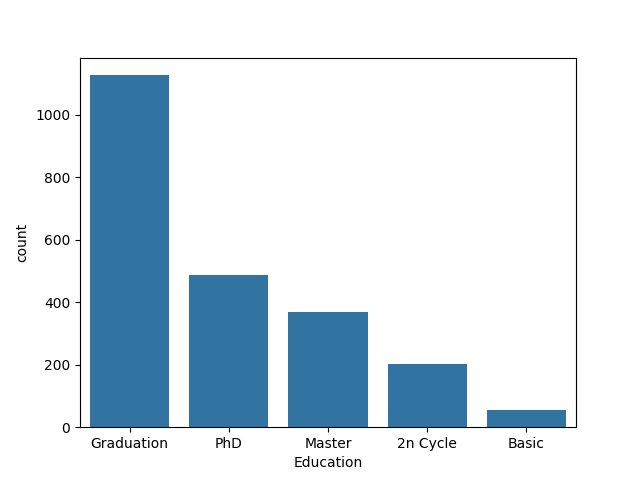
\includegraphics[width=\linewidth]{figures/education_barplot.png}
%     \caption{Bar plot of value counts of the Education column}
%     \label{fig:educ bar}
% \end{figure}

\subsubsection{Bivariate Analysis}

The relationships of attributes to each other are also worth considering to look at. Given that a lot of the analysis of these attributes would later be interpreted by the models which will be seen at the discussion.

Looking at the scatterplot for the income per year of birth, ignoring the outliers, it seems that there seems to be an equal distribution for each year. Looking around the years 1970 to 1980, there seems to be a few entries where the recorded income is higher than the usual. 

\begin{figure}[H]
    \centering
    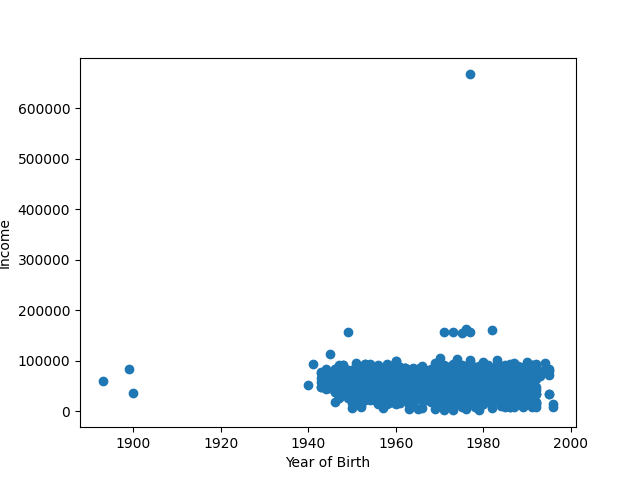
\includegraphics[width=\linewidth]{figures/income_per_yob.png}
    \caption{Scatterplot of income per year of birth}
\end{figure}

Regarding education, when categorized and calculated for central tendencies, \texttt{Basic} provides the lowest average income, while a \texttt{PhD} provides the highest average. However, according to table \ref{tab:educ mean std}, Basic education seems to be the most stable when it comes to delivering a salary based on the standard deviation. PhD education, although high in the average salary, is also very high in standard deviation. This could be seen at the $min$ and $max$ of each category where the minimum income of someone with PhD degree can be as low as 4023 while someone with basic education can be sure to have a salary that is atleast 7500.

\begin{table}[H]
    \caption{Descriptive statistics for each unique value in the Education column}
    \label{tab:educ mean std}
    \begin{tabularx}{\linewidth}{l|>{\centering}X>{\centering}X>{\centering}X>{\centering\arraybackslash}X}
        \toprule
        Education & $\bar x$ & $\sigma$ & min & max \\
        \midrule
        2n Cycle & 47633.19 & 22119.08 & 7500 & 96547\\
        Basic & 20306.26 & 6235.07 & 7500 & 34445\\
        Graduation & 52720.37 & 28177.19 & 1730 & 666666\\
        Master & 52917.53 & 20157.79 & 6560 & 157733\\
        PhD & 56145.31 & 20612.98 & 4023 & 162397\\
        \bottomrule
    \end{tabularx}
\end{table}
